%! TEX program = xelatex
\documentclass{report}
% provides basic settings for ctex document
\usepackage[UTF8, heading=true]{ctex}
\usepackage{fancyhdr}
\usepackage{tocloft}
\usepackage[margin=1in]{geometry}
\usepackage{metalogo}                   % \XeLaTeX
\usepackage{float}                      % figure H flag
\usepackage{microtype}                  % break long words
\usepackage[hidelinks]{hyperref}
\usepackage{tabularx}
\usepackage{amsmath}
\usepackage{lmodern}                    % allow fonts to scale
\usepackage{placeins}
\usepackage{multirow}                   % multirow, multicolumn support
\usepackage{booktabs}                   % toprule, cmidrule support
\usepackage{caption}

% make chapter stay in the same page
%\makeatletter
%\renewcommand\chapter{\thispagestyle{plain}%
%\global\@topnum\z@
%\@afterindentfalse
%\secdef\@chapter\@schapter}
%\makeatother

\fancyhead{}
\renewcommand{\sectionmark}[1]{\markleft{#1}}
\renewcommand{\partmark}[1]{\markright{#1}}
\lhead{\leftmark}
\rhead{\rightmark}
% see $(texdoc ctex) for details
\ctexset{
    chapter = {
        format += \flushleft,
        number = \arabic{chapter},
    },
    section = {
        format += \flushleft,
    },
    appendix = {
        number = \Alph{chapter},
        name = {附录},
    },
}

\pagestyle{fancy}

%\setlength\cftaftertoctitleskip{2em}

% provides code input support
\usepackage{xparse}                     % newcommand multiple optional arguments
\usepackage{listings}                   % code
\usepackage{fontspec}
\usepackage{lmodern}

%\newfontfamily\codeF{Fira Code}

\setmonofont[
    Contextuals={Alternate},
    ItalicFont = Fira Code      % to avoid font warning
]{Fira Code}

% usage: \inputCode{[language] <path>}
% if language is not explicitly set, it's defaulted to c
\DeclareDocumentCommand{\inputCode}{ O{c} m }{
    {
        \lstinputlisting[
            basicstyle=\small\ttfamily,
            language={#1},
            tabsize=4,
            showstringspaces=false,
            breaklines=true,
            frame=shadowbox,
            framexleftmargin=10mm,
            rulesepcolor=\color{black},
            numbers=left,
            xleftmargin=4em,
        ]{#2}
    }
}

\DeclareDocumentCommand{\inputCodeSetLanguage}{ m }{
    \lstset{
        basicstyle=\small\ttfamily,
        language={#1},
        tabsize=4,
        showstringspaces=false,
        breaklines=true,
        frame=shadowbox,
        framexleftmargin=10mm,
        rulesepcolor=\color{black},
        numbers=left,
        xleftmargin=4em,
    }
}



%%%%%%%%%%%%%%%%%%%%%%%%%%%%%%%%
\graphicspath{{./res/}}

% report content %%%%%%%%%%%%
%%%%%%%%%%%%%%%%%%%%%%%%%%%%%
\begin{document}

% cover page
\begin{titlepage}
    \addtolength{\topmargin}{1cm}
    \centering
    
\includegraphics[width=0.6\textwidth]{hust.jpg}\par
    \vspace{0.5cm}
    {\Huge \heiti 操作系统课程设计报告}\par
    \vspace{10cm}
    {
        \large
        \begin{tabular}{r m{8em}}
            \makebox[6em][s]{学生姓名}:& 胡思勖 \\ \cline{2-2}
            %\makebox[6em][s]{学生姓名}:& 陈志浩 \\ \cline{2-2}
            %\makebox[6em][s]{学生姓名}:& 黄志强\\ \cline{2-2}
            \makebox[6em][s]{学号}:& U201514898\\ \cline{2-2}
            %\makebox[6em][s]{学号}:& U201514893\\ \cline{2-2}
            %\makebox[6em][s]{学号}:& U201514896\\ \cline{2-2}
            \makebox[6em][s]{专业}:& 计算机科学与技术\\ \cline{2-2}
            \makebox[6em][s]{班级}:& 计卓1501\\ \cline{2-2}
            \makebox[6em][s]{指导教师}:& 张杰 \\ \cline{2-2}
        \end{tabular}
    }
    \vfill
    2018-03-03
\end{titlepage}

\setcounter{tocdepth}{1}
\pagenumbering{Roman}
\tableofcontents

\newpage
\pagenumbering{arabic}
\setcounter{page}{1}



% chapter 1
\chapter{Booting a PC}
\label{cha:booting_a_pc}

\section{PC Bootstrap}
\par 这一部分主要介绍了x86语言以及PC的启动过程,并让我们熟悉了QEMU和GDB的调试方法。

\subsection{Getting Started with x86 assembly}
\par 通过阅读\emph{PC Assembly Language Book}\footnote{\url{https://pdos.csail.mit.edu/6.828/2017/readings/pcasm-book.pdf}}来学习x86的语法。注意这本书值使用的NASM汇编,但是实验中使用的是GNU的AT\&T语法。



% chapter 2
\chapter{基于pthread的形态学图像处理}
\section{实验目的与要求}
\begin{itemize}
    \item 掌握使用pthread的基本的并行编程设计方法以及调优方法;
    \item 掌握并行编程中基本的数据分块以及任务分解的方法。
    \item 使用pthread实现并行的形态学图像处理。
    \item 简要分析以及总结处理的结果。
\end{itemize}

\section{算法描述}
\par 使用多个线程对于一个图像进行蚀刻以及膨胀的算法如下,算法为一个线程的流程,而有多个这样的线程同时进行。
\begin{simpleAlgorithm}{pthread并行处理算法(一个线程)}
    \Procedure{PthreadParallel}{$blocks$}
    \While{true}
        \State lock\((blocks)\)
        \State get first block \(blk\) from \(blocks\)
        \If{\(blocks\).empty()}
            \State unlock\((blocks)\)
            \State \Return
        \EndIf
        \State unlock\((blocks)\)
        \State \Call{ErodeAndDilate}{$blk, kernel_e, kernel_d$}
    \EndWhile
    \EndProcedure
\end{simpleAlgorithm}
\par 算法中,\(blocks\)参数为一个工作队列,队列中的工作为原预处理过后的图片的子图片。在每个线程的每个循环中,首先锁住队列,从队列中获取一个子图片\(blk\)、解锁队列然后使用上一章中的ErodeAndDilate过程进行处理。如果\(blocks\)中没有子图片,说明处理完成,则此线程退出。
\par 主线程的流程如图\ref{fig:pthreadMain}所示。在进行预处理过后启动多个线程,然后等待所有线程竞争子图像、处理然后结束即可,最后保存处理的结果即可。
\begin{figure}[htpb]
    \centering
    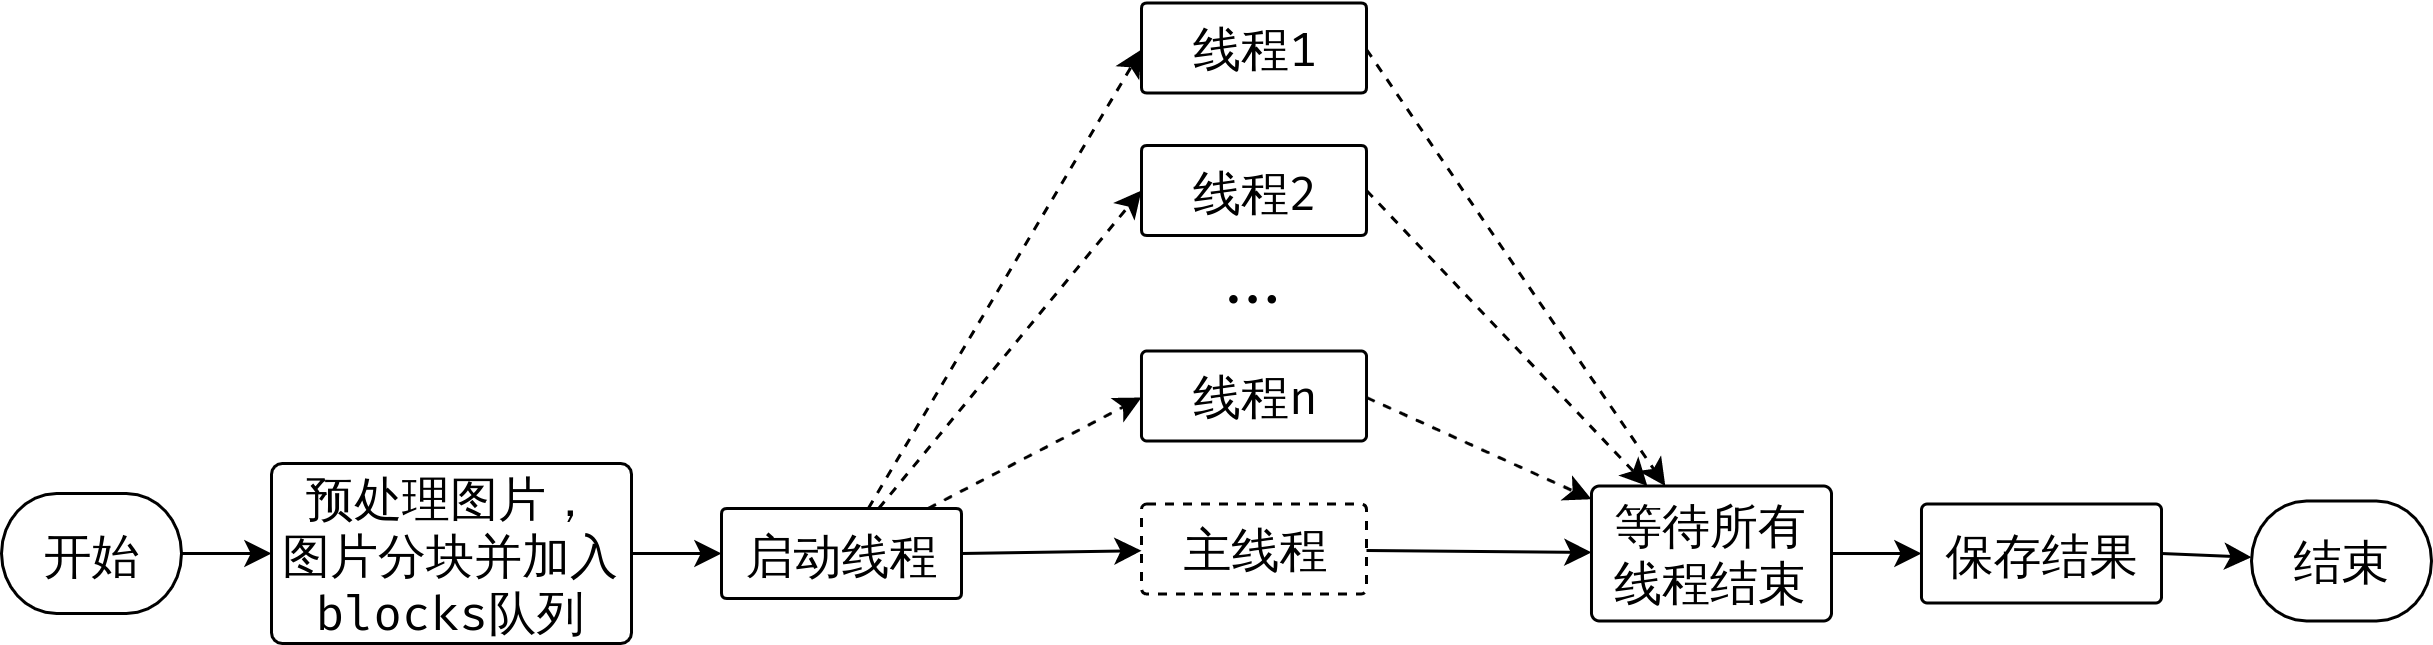
\includegraphics[width=0.95\linewidth]{pthreadMain.png}
    \caption{主线程流程}
    \label{fig:pthreadMain}
\end{figure}

\par 由于是使用pthread的并行算法,每一个线程处理一个部分,因此首先需要将数据分块(即分为算法中的\(blocks\))。分块方式如图\ref{fig:partition}所示。每块大小一样,在边缘部分如果块大小不符则按照原图的边缘进行裁减。因此,在进行处理时需要对于边缘部分进行考虑。
\begin{figure}[htpb]
    \centering
    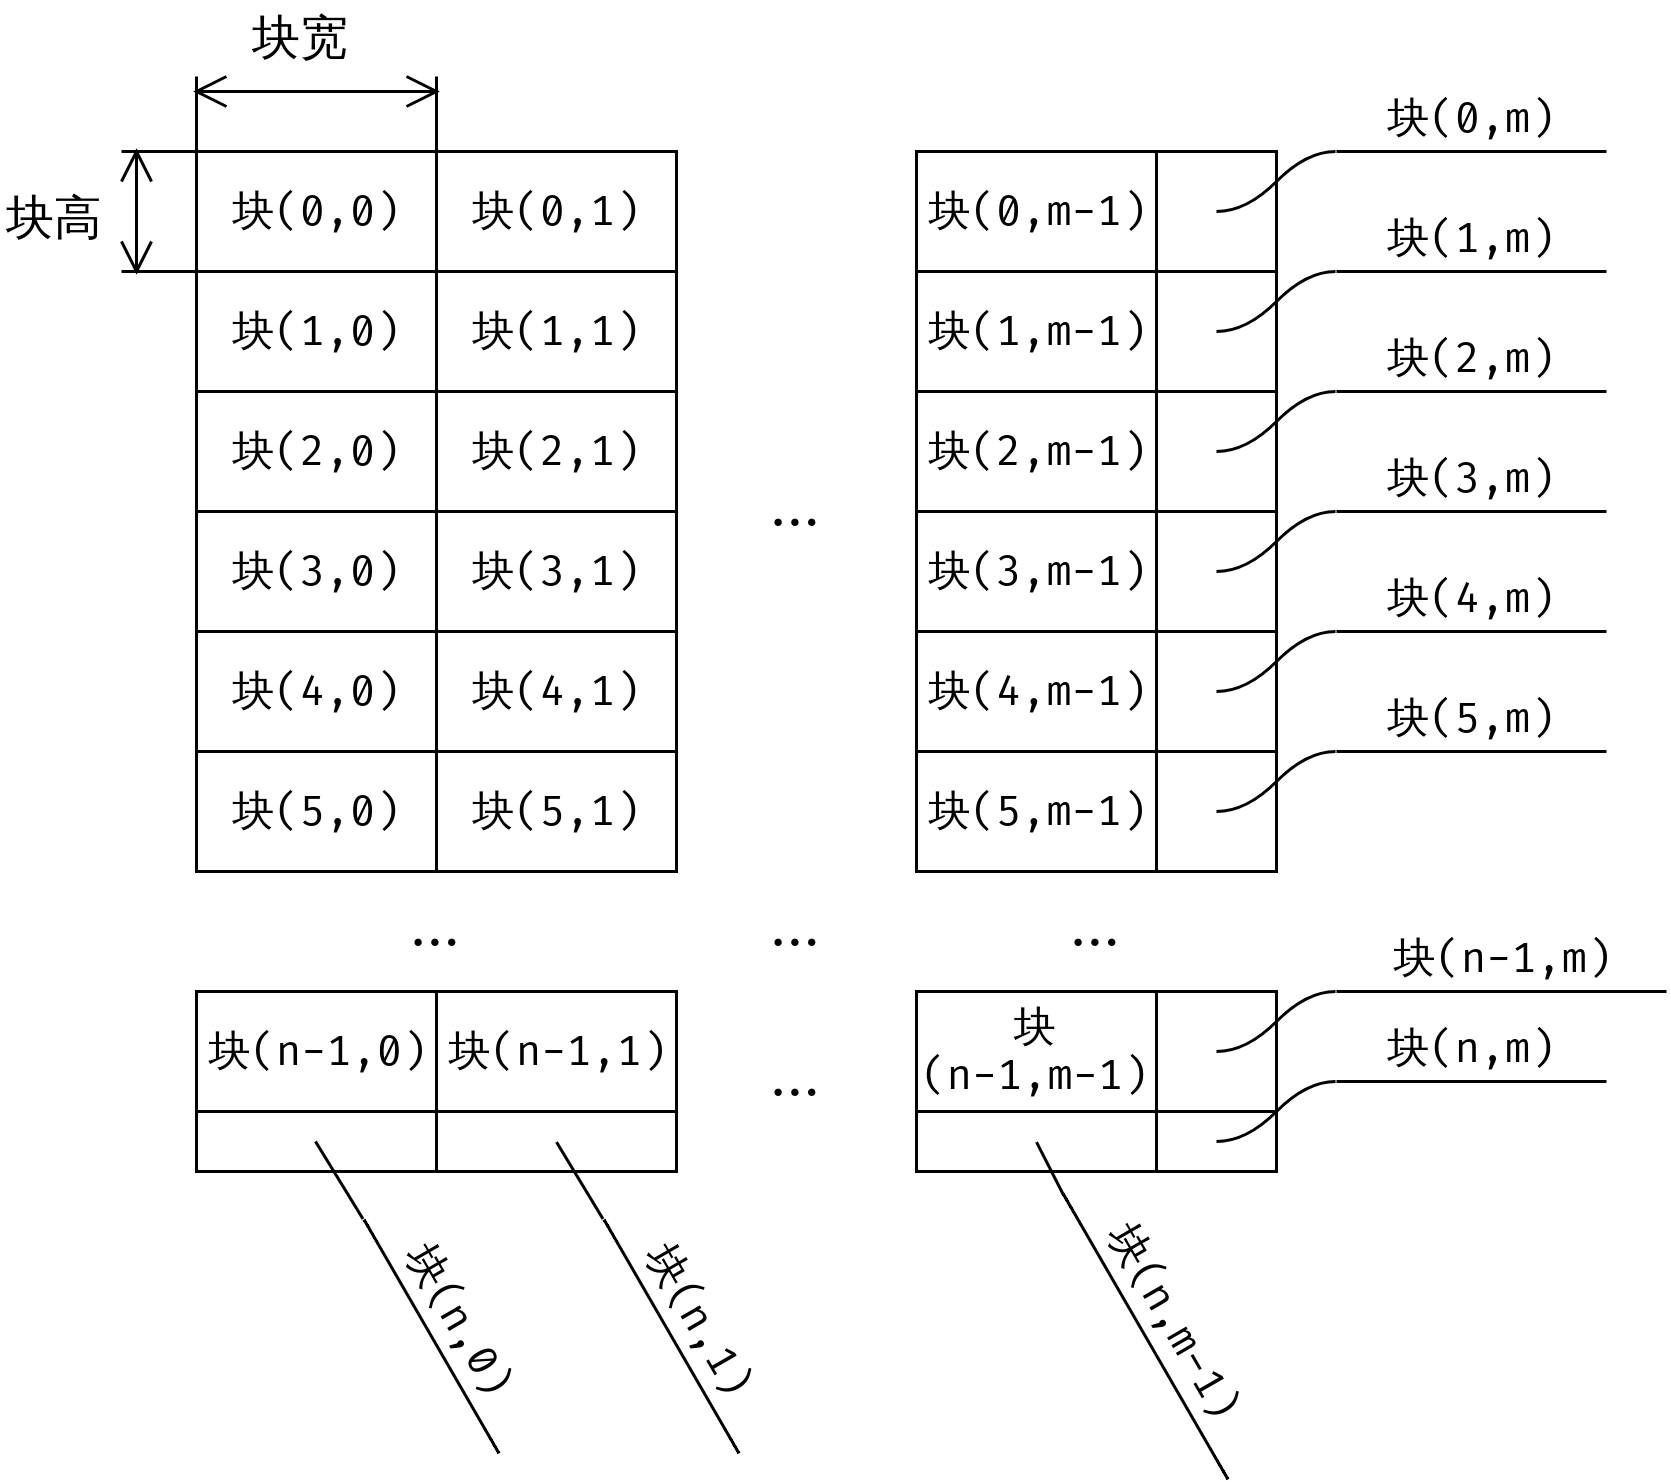
\includegraphics[width=0.76\linewidth]{partition.png}
    \caption{分块方法}
    \label{fig:partition}
\end{figure}

\section{实验方案}
\par 所有的开发与运行环境见附录\ref{cha:env},表\ref{tab:env},此后实验的开发与运行环境均相同,不再赘述。根据算法描述、分块方法以及主线程的流程编写程序并运行,然后观察结果并与串行的程序比较。经过多轮的比较以及参数调试后得出一个较好的效果。

\section{实验结果与分析}
\par 功能上,程序处理后的图片与串行处理后的图片一致,此处不再给出。4线程,分块大小为128的情况下程序的运行时间如图\ref{fig:pthreadOutput}所示。在4个线程的情况下,运行三次的平均运行时间为11.7s,相比于串行算法,程序的加速比为\(44.2\div 11.7 = 3.77\),已经十分接近理想加速比4。
\begin{figure}[htpb]
    \centering
    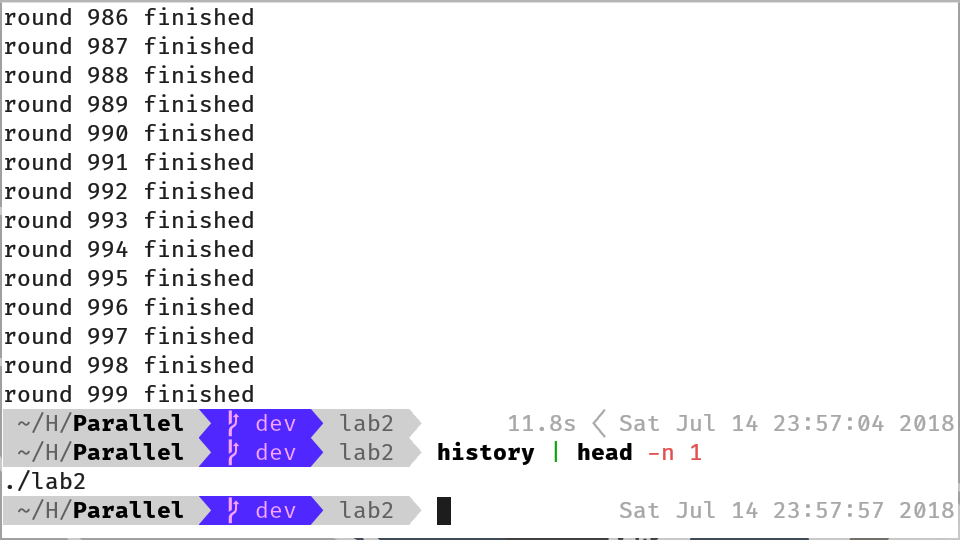
\includegraphics[width=0.9\linewidth]{pthreadOutput.png}
    \caption{pthread程序运行时间}
    \label{fig:pthreadOutput}
\end{figure}

\par 经过8组、每组3次的测试,加速比随线程变化的曲线如图\ref{fig:pthreadTrend}所示。可以看出,在线程数为1\textasciitilde 4时加速比随着线程数几乎呈线性变化,而在线程数为1时加速比为1.006,overhead所占用的时间几乎可以不计。在线程数达到4时由于物理内核已经被占满,因此后面加速比不再增加,随着线程数量的进一步增大,由于线程调度的开销,因此程序的加速比不再增加,反而有所下降。
\begin{figure}[htpb]
    \centering
    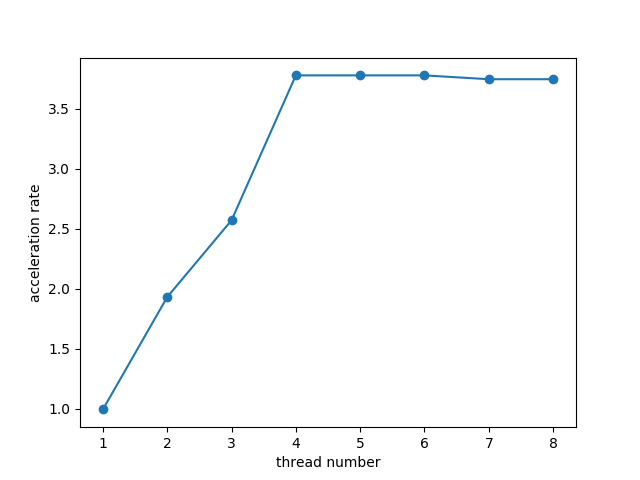
\includegraphics[width=0.8\linewidth]{pthreadTrend.png}
    \caption{加速比随线程数变化}
    \label{fig:pthreadTrend}
\end{figure}

\par 对于分块大小而言,加速比随着分块大小的变化如图\ref{fig:pthreadTrend2}所示,在分块大小较小时,加速比随着分块大小的变化并不大,只在分块大小过小时由于线程调度导致一点性能开销。当分块大小大于原图的一半时总时间则取决于分到最大分块线程所用的时间,因此在这个区间内性能随分块大小呈下降趋势。
\begin{figure}[htpb]
    \centering
    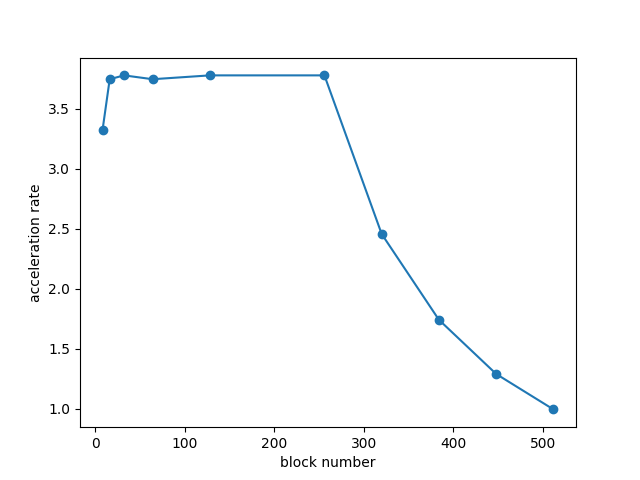
\includegraphics[width=0.8\linewidth]{pthreadTrend2.png}
    \caption{加速比随分块大小变化}
    \label{fig:pthreadTrend2}
\end{figure}




\chapter*{心得体会}
\addcontentsline{toc}{chapter}{心得体会}
\label{cha:xin_de_ti_hui_}

\par 通过这次实验,我对于cache的结构,运作方式以及如何更高效的写出cache friendly的代码有了更为深入的了解。通过对于cache的模拟,我对于cache的组成方式,与内存地址的对应关系以及cache组相连的工作方式有了更为深入的认识。
\par 在对于错误代码的调试过程中,我尝试使用了各种方法来结构性的显示cache的内容以及替换的过程,这也给了我有关cache工作方式更为直观的印象。
\par 第二个实验则更令我印象深刻,它从简单的矩阵变换入手,展示了对于程序员而言透明的cache是如何影响代码性能的,以及程序员应该如何优化代码使之能够在cache层面有更好的工作效率。通过逐步深入的实验,对于cache的理解也逐步加深,并在实验查阅资料的过程中了解到了cache优化在包括科学计算等多个领域的应用,这不仅开拓了我的视野,也为今后的学习工作奠定了基础。

{\let\clearpage\relax \chapter*{源代码}}
\addcontentsline{toc}{chapter}{源代码}
\label{cha:yuan_dai_ma_}

\inputCodeSetLanguage{c}
\noindent \textbf{csim.c}
\lstinputlisting{../src/csim.c}

\noindent \textbf{trans.c}
\lstinputlisting{../src/trans.c}

\vfill
{\tiny written by HuSixu \hfill powered by \XeLaTeX .}
\end{document}

%%%%%%%%%%%%%%%%%%%%%%%%%%%%%%%%%%%%
%%%%%%%%%%%%%%%%%%%%%%%%%%%%%%%%%%%%
%%%%%%%%%%%%%%%%%%%%%%%%%%%%%%%%%%%%
% in this report i learned:
% how to use a tcolorbox(see conf/report_settings.tex)
% how to use a siderule(see conf/report_settings.tex)
% how to use long argument in xparse (+m, +o, ..., see cont/report_settings.tex)
% how to use latex and avoid warning(see conf/ctex_wrapper.tex)
% how to use footnote in a box and let footnote show at the bottom of the page (use footnotemark and footnotetext, do not use footmisc package)

